\documentclass[openany,twoside, notitlepage,letterpaper,11pt]{book}

%%% These are the packages that are used
%used for custom page headers and page numbering
\usepackage{fancyhdr}

%adds TeX fonts from the American Mathematical Society.
\usepackage{amsfonts}

%Sets the bounds of the page margins
\usepackage[top=1in, bottom=1in, left=0.7in, right=.7in]{geometry}

%Various useful packages
\usepackage{amsmath,amssymb, amscd,amsbsy, amsthm, enumerate}
\usepackage{mdframed, titlesec, setspace,verbatim, multicol, caption}
\usepackage[unicode]{hyperref}
\usepackage{wasysym}
\usepackage{tikz, polynom}
\usepackage{xcolor}
\usepackage{etoolbox}

%enables the ability of including pages from a pdf.
\usepackage{pdfpages}

%enables drawings of circuit diagrams
\usepackage{circuitikz}

%enables indexing
\usepackage{makeidx} 

%enables changing the bibliography name
\usepackage[nottoc,notlof,notlot]{tocbibind}

%makes the index size footnote
\usepackage[font=footnotesize, columns=3]{idxlayout}

%Adds extra symbols
\usepackage{mathrsfs, upgreek}

%Allows for tables with cells that span multiple rows and columns
\usepackage{multirow}



%This is where settings for the latex file are stored.
%%Version Number
\newcommand{\Version}{0.001}
%%Version

%%% Page formatting
%\setlength{\headsep}{30pt}
\setlength{\parindent}{25pt}
\setlength{\textheight}{9in}

%Rename the bibliography to References.
\renewcommand\bibname{References}


%%% Header and Footer Info
\pagestyle{fancy}
\fancyhead[LO]{\small {\textbf{Antonius' Compendium -- Volume I. Version \Version}}}
\fancyhead[RE]{\small {\textbf{Antonius' Compendium -- Volume I. Version \Version}}}
\fancyhead[C]{}
\fancyhead[RO]{\small \thepage}
\fancyhead[LE]{\small \thepage}
\fancyfoot[L]{}
\fancyfoot[C]{}
\fancyfoot[R]{}


\patchcmd{\chapter}{plain}{empty}{}{}
\titleformat{\chapter}[display]
{\normalfont\huge\bfseries}{}{0pt}{\Huge}
\titlespacing*{\chapter} {0pt}{-50pt}{10pt}

%re-defines the plain page style
\fancypagestyle{plain}{%
	\fancyhf{}
	\rhead{\thepage}
	\renewcommand{\headrulewidth}{0pt}}

%This is where custom definitions and variables are defined and stored.
\newcommand{\andspace}[1]{\hspace{#1}\textrm{and}\hspace{#1}}

\numberwithin{equation}{section}
\setlength{\columnsep}{.5cm}
\setlength{\columnseprule}{1pt}
\def\columnseprulecolor{\color{black}}

\newcommand{\abs}[1]{\left| #1 \right|}
\newcommand{\inner}[1]{\langle #1 \rangle}
\newcommand{\norm}[1]{\left\lVert#1\right\rVert}
\newcommand{\spanvect}{\textnormal{span}}
\newcommand{\union}{\cup}
\newcommand{\Union}{\bigcup}

% Defines a keyword which will bold and add a word to the index.
\newcommand{\keyword}[1]{\textbf{#1}\index{#1}}

% Create a section without making the section title.
\newcommand\invisiblesection[1]{%
	\refstepcounter{section}%
	\addcontentsline{toc}{section}{\protect\numberline{\thesection}#1}%
	\sectionmark{#1}}

% Makes a chapter with no title
\makeatletter
\newcommand{\unchapter}[1]{%
	\begingroup
	\let\@makechapterhead\@gobble % make \@makechapterhead do nothing
	\chapter{#1}
	\endgroup
}
\makeatother

%%% These are some shortcuts that are handy
\def\real{{\mathbb R}}
\def\Natural{\mathbb{N}}
\def\dx{\textnormal{dx}}
\def\dy{\textnormal{dy}}
\def\dz{\textnormal{dz}}
\def\dt{\textnormal{dt}}
\def\ds{\textnormal{ds}}
\def\dw{\textnormal{dw}}
\def\Re{\textnormal{Re}}
\def\Im{\textnormal{Im}}
\def\exp{\textnormal{exp}}
\def\interior{\textnormal{interior}}
\def\al{\alpha}
\def\del{\delta}
\def\Del{\Delta}
\def\gam{\gamma}
\def\Gam{\Gamma}
\def\Om{\Omega}
\def\ep{\varepsilon}
\def\lam{\lambda}
\def\rational{{\mathbb Q}}
\def\integer{{\mathbb Z}}
\def\Q{{\mathbb Q}}
\def\Z{{\mathbb Z}}
\def\N{{\mathbb N}}
\def\R{{\mathbb R}}
\def\grad{\nabla}
\def\C{\mathcal C}
\def\P{\mathcal P}
\def\T{\mathcal T}
\def\I{\mathcal I}
\def\intersect{\cap}
\def\Intersect{\bigcap}


%%% This defines the solution environment for you to write your solutions
\newenvironment{soln}
{\let\oldqedsymbol=\qedsymbol
	\renewcommand{\qedsymbol}{$ $}
	\begin{proof}[\bfseries\upshape \color{blue}Derivation]\color{blue}}
	{\end{proof}
	\renewcommand{\qedsymbol}{\oldqedsymbol}}

\newenvironment{note}
{\let\oldqedsymbol=\qedsymbol
	\renewcommand{\qedsymbol}{$ $}
	\begin{proof}[\bfseries\upshape \color{red}Note]\color{red}}
	{\end{proof}
	\renewcommand{\qedsymbol}{\oldqedsymbol}}
	

\newenvironment{Deletion}
{\let\oldqedsymbol=\qedsymbol
	\renewcommand{\qedsymbol}{$ $}
	\begin{proof}[\bfseries\upshape \color{red}Deletion]\color{red}}
	{\end{proof}
	\renewcommand{\qedsymbol}{\oldqedsymbol}}


%theorem
\newcounter{theo}[section] \setcounter{theo}{0}
\renewcommand{\thetheo}{\arabic{chapter}.\arabic{section}.\arabic{theo}}
\newenvironment{theo}[2][]{%
	\refstepcounter{theo}%
	\ifstrempty{#1}%
	{\mdfsetup{%
			frametitle={%
				\tikz[baseline=(current bounding box.east),outer sep=0pt]
				\node[anchor=east,rectangle,fill=blue!20]
				{\strut Theorem~\thetheo};}}
	}%
	{\mdfsetup{%
			frametitle={%
				\tikz[baseline=(current bounding box.east),outer sep=0pt]
				\node[anchor=east,rectangle,fill=blue!20]
				{\strut Theorem~\thetheo:~#1};}}%
	}%
	\mdfsetup{innertopmargin=10pt,linecolor=blue!20,%
		linewidth=2pt,topline=true,%
		frametitleaboveskip=\dimexpr-\ht\strutbox\relax
	}
	\begin{mdframed}[]\relax%
		\label{#2}}{\end{mdframed}}
%%%%%%%%%%%%%%%%%%%%%%%%%%%%%%

%Lemma
\newcounter{lemm}[section] \setcounter{lemm}{0}
\renewcommand{\thelemm}{\arabic{chapter}.\arabic{section}.\arabic{lemm}}
\newenvironment{lemm}[2][]{%
	\refstepcounter{lemm}%
	\ifstrempty{#1}%
	{\mdfsetup{%
			frametitle={%
				\tikz[baseline=(current bounding box.east),outer sep=0pt]
				\node[anchor=east,rectangle,fill=green!20]
				{\strut Lemma~\thelem};}}
	}%
	{\mdfsetup{%
			frametitle={%
				\tikz[baseline=(current bounding box.east),outer sep=0pt]
				\node[anchor=east,rectangle,fill=green!20]
				{\strut Lemma~\thelem:~#1};}}%
	}%
	\mdfsetup{innertopmargin=10pt,linecolor=green!20,%
		linewidth=2pt,topline=true,%
		frametitleaboveskip=\dimexpr-\ht\strutbox\relax
	}
	\begin{mdframed}[]\relax%
		\label{#2}}{\end{mdframed}}
%%%%%%%%%%%%%%%%%%%%%%%%%%%%%%

%Proof
\newcounter{prf}[section]\setcounter{prf}{0}
\renewcommand{\theprf}{\arabic{chapter}.\arabic{section}.\arabic{prf}}
\newenvironment{prf}[2][]{%
	\refstepcounter{prf}%
	\ifstrempty{#1}%
	{\mdfsetup{%
			frametitle={%
				\tikz[baseline=(current bounding box.east),outer sep=0pt]
				\node[anchor=east,rectangle,fill=red!20]
				{\strut Proof~\theprf};}}
	}%
	{\mdfsetup{%
			frametitle={%
				\tikz[baseline=(current bounding box.east),outer sep=0pt]
				\node[anchor=east,rectangle,fill=red!20]
				{\strut Proof~\theprf:~#1};}}%
	}%
	\mdfsetup{innertopmargin=10pt,linecolor=red!20,%
		linewidth=2pt,topline=true,%
		frametitleaboveskip=\dimexpr-\ht\strutbox\relax
	}
	\begin{mdframed}[]\relax%
		\label{#2}}{\qed\end{mdframed}}
%%%%%%%%%%%%%%%%%%%%%%%%%%%%%%

%Definition
\newcounter{defn}[section] \setcounter{defn}{0}
\renewcommand{\thedefn}{\arabic{chapter}.\arabic{section}.\arabic{defn}}
\newenvironment{defn}[2][]{%
	\refstepcounter{defn}%
	\ifstrempty{#1}%
	{\mdfsetup{%
			frametitle={%
				\tikz[baseline=(current bounding box.east),outer sep=0pt]
				\node[anchor=east,rectangle,fill=gray!20]
				{\strut Definition~\thedefn};}}
	}%
	{\mdfsetup{%
			frametitle={%
				\tikz[baseline=(current bounding box.east),outer sep=0pt]
				\node[anchor=east,rectangle,fill=gray!20]
				{\strut Definition~\thedefn:~#1};}}%
	}%
	\mdfsetup{innertopmargin=10pt,linecolor=gray!20,%
		linewidth=2pt,topline=true,%
		frametitleaboveskip=\dimexpr-\ht\strutbox\relax
	}
	\begin{mdframed}[nobreak=true]\relax%
		\label{#2}}{\end{mdframed}}
	
%Fancy Box
\newcounter{fancybox}[section] \setcounter{fancybox}{0}
\renewcommand{\thefancybox}{\arabic{chapter}.\arabic{section}.\arabic{fancybox}}
\newenvironment{fancybox}[2][]{%
	\refstepcounter{fancybox}%
	\ifstrempty{#1}%
	{\mdfsetup{%
			frametitle={%
				\tikz[baseline=(current bounding box.east),outer sep=0pt]
				\node[anchor=east,rectangle,fill=orange!20]
				{\strut ~\thefancybox};}}
	}%
	{\mdfsetup{%
			frametitle={%
				\tikz[baseline=(current bounding box.east),outer sep=0pt]
				\node[anchor=east,rectangle,fill=orange!20]
				{\strut ~\thefancybox:~#1};}}%
	}%
	\mdfsetup{innertopmargin=10pt,linecolor=orange!20,%
		linewidth=2pt,topline=true,%
		frametitleaboveskip=\dimexpr-\ht\strutbox\relax
	}
	\begin{mdframed}[]\relax%
		\label{#2}}{\end{mdframed}}


%creates the title page
\title{
\includegraphics[scale=2.5]{./Images/Covers/AC.png}
	\\ Compendium of Knowledge \\ Volume II: Neural Nucleus \\ Version \Version}
\date{}
\author{Compiled by: Antonius W. Torode$^{1}$ \\ \scriptsize{1. Applied Research Laboratories - University Of Texas: Austin} \\ Written in: \LaTeX}

\makeindex
%\addcontentsline{toc}{chapter}{Index}


%%% Document Starts now
\begin{document}

%Begin the front matter.
\frontmatter
%Begins title page.	
\maketitle
\thispagestyle{empty}
\pagestyle{empty}
\begin{center}	
	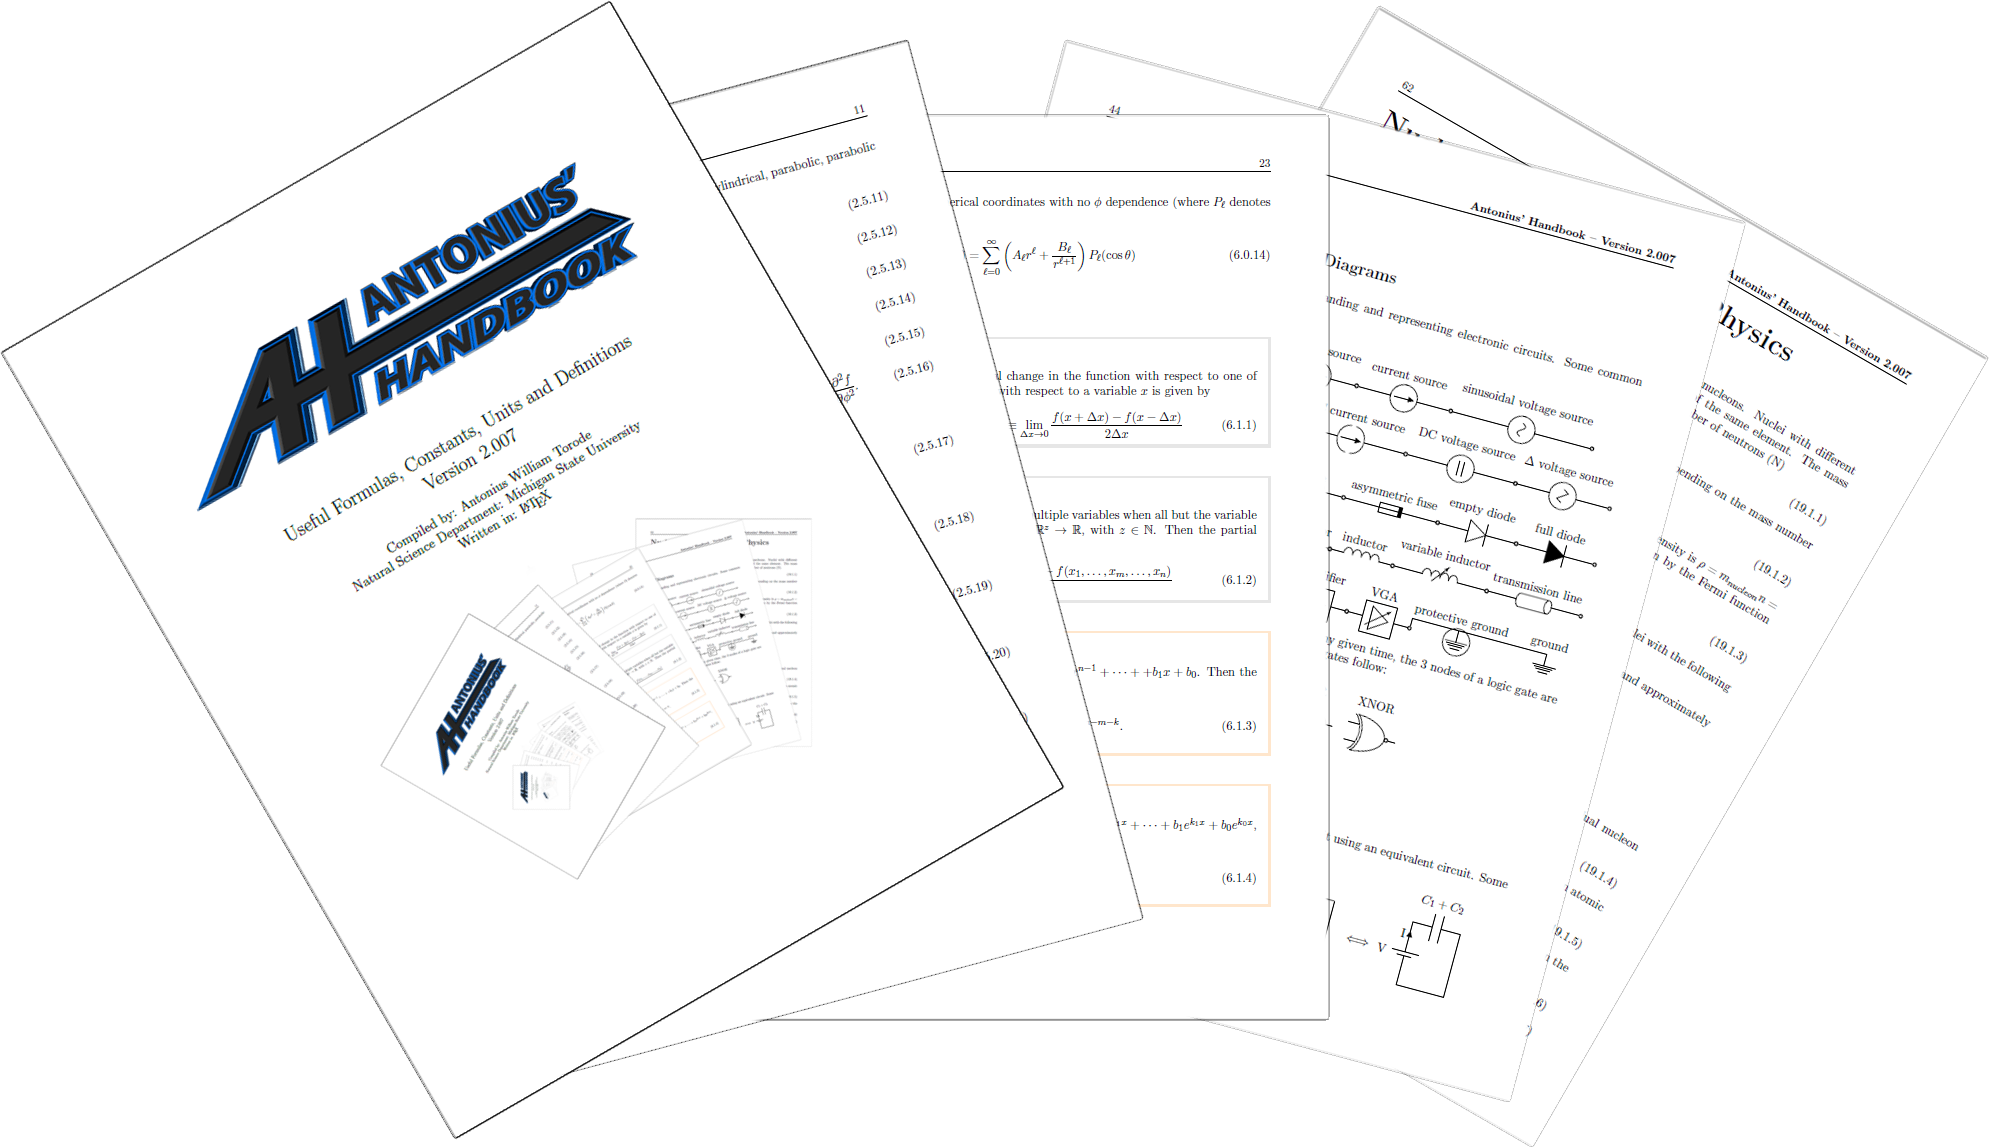
\includegraphics[scale=1.6]{./Images/Covers/background_tunnel.png}
\end{center}

%Copywrite page
\pagestyle{empty}
%% copyrightpage
\begingroup
\footnotesize
\parindent 0pt
\parskip \baselineskip
\textcopyright{} 2025 Antonius Torode \\
All rights reserved.

This work may be distributed and/or modified under the conditions of Antonius’ General Purpose License (AGPL).

The original maintainer of this work is: Antonius Torode.

The current maintainer of this work is: Antonius Torode.


Chief Editor: Antonius Torode

%\hfill\begin{minipage}{\textwidth-1cm}Other contributors:\end{minipage}

Published by Antonius Torode. 

Hosted at: https://torodean.github.io/

Github Repository: https://github.com/torodean/Antonius-Compendium

%\begin{center}
%\begin{tabular}{ll}
%First Personal Release (Version 0.000): & January 2016 \\
%First Public Release (Version 1.000): &  July 2016 \\
%Most Current Revision Date (Version \Version): & \today 
%\end{tabular}
%\end{center}

\vfill

Torode, A.\\
\hspace*{1em} Antonius' Compendium. \\
\hspace*{2em} Applied Research Laboratories -- \\
\hspace*{2em} \today \\
\hspace*{2em} Volume II. \\
\hspace*{2em} Version: \Version



\endgroup
\clearpage

%Preface page
\begin{center}
	\textbf{Preface}
\end{center}

This document is a compilation of ideas, scratch work, derivations, useful formulas, definitions, constants, and general information used for my own studies as a reference while furthering self education. These are my notes. It's purpose is to provide a complete 'compendium' per say of various ideas used often. All the material in this document was either directly copied from one of the references listed at the end or derived from scratch. On occasion \textit{typos may exist} due to human error but will be corrected when discovered.
	
The version number is updated every time the document is distributed, printed for distribution, or a major update is added. This ensures that there is no two copies with different information and similar version numbers. The latest update date is automatically set to the current date each time the document is edited. Please refrain from distributing this handbook without permission from the original author/compiler. This book is formatted for printing.

\begin{center}
	\textbf{Topics Covered In This Book}
\end{center}

\begin{multicols}{2}
\begin{itemize}
	\item Machine Learning
	\item Artificial Intelligence
	\item Modeling
	\item Psychology
\end{itemize} 
\end{multicols}

The information in this book is in no way limited to the topics listed above. They serve as a simple guideline to what you will find within this document. For more information about this book or details about how to obtain your own copy please visit:
\begin{center}
	https://torodean.github.io/
\end{center}

\begin{quotation}
``Scientific theories deal with concepts, not with reality. All theoretical results are derived from certain axioms by deductive logic. In physical sciences the theories are so formulated as to correspond in some useful sense to the real world, whatever that may mean. However, this correspondence is approximate, and the physical justification of all theoretical conclusions is based on some form of inductive reasoning.'' - Athanasios Papoulis (Probability, Random Variables, and Stochastic Processes book)
\end{quotation}

\begin{center}
	\textbf{Disclaimer}
\end{center}

This book contains formulas, definitions, and theorems that by nature are very precise. Due to this, some of the material in this book was taken directly from other sources such as but not limited to Wolfram Mathworld. This is only such in cases where a change in wording could cause ambiguities or loss of information quality.  Following this, all sources used are listed in the references section and cited when used.


%Begins blank page.
\thispagestyle{empty}
\newpage
\vspace*{\stretch{1}}
\begin{center}
	\textit{This page intentionally left blank.\\ (Yes, this is a contradiction.)}
\end{center}
\vspace*{\stretch{1}}

%Begins table of contents
\tableofcontents


%Begin the mainmatter.
\setlength{\parindent}{0pt}
\mainmatter
\pagestyle{fancy}
%\chapter{Constants and units}
\thispagestyle{fancy}
\begin{fancybox}[Physical Constants]{}	
\begin{center}
	\begin{tabular}{   l  |  c  |  l  |  l  }
		Constant & Symbol & Value & Units \\
		\hline
		Speed of light in a vacuum& c $\equiv 1/\sqrt{\mu_0\epsilon_0}$ & $2.99792458 \times 10^8$ & m/s \\
		Elementary charge& e & $1.602176565(35)\times 10^{-19}$ & C\\
		Gravitational constant& G & $6.67384(80)\times 10^{-11}$ & m$^3$kg$^{-1}$s$^{-2}$\\
		Avagadro's number& $N_a$ & $6.02214129(27)\times 10^{23}$ & mol$\cdot s^{-1}$\\
		Planck constant & $h$ & $ 6.62606872(52) \times 10^{-34}$ & J$\cdot$s \\
		& & $4.135668 \times 10^{-15}$ & eV$\cdot$s \\
		& $hc$ & 1239.84 & eV$\cdot$nm \\
		Reduced planck constant& $\hbar \equiv h/2\pi$ & $1.05\times 10^-{34}$ & J$\cdot$s\\
		Permittivity of the vacuum & $\epsilon_0$ & $8.854\times 10^{-12}$ & C$^2$N$^{-1}$m$^{-2}$ \\
		Permeability of the vacuum & $\mu_0$ & $4\pi\times 10^{-7}$ & N/A$^{2}$ \\
		Permeability of the vacuum & $\mu_0$ & $4\pi\times 10^{-7}$ & N/A$^2$ \\
		Boltzmann constant & $k_B$ & $1.38064852\times 10^{-23}$ & J/K \\
				 & & $8.61733\times 10^{-5}$ & eV/K \\
		Stefan-Boltzmann constant & $\sigma_{\textrm{B}} \equiv \frac{\pi^2k_B^4}{60\hbar^3c^3}$ & $5.670367(13)\times 10^{-8}$ & W$\cdot$m$^{-2}$K$^{-4}$ \\
		Thomson cross-section & $\sigma_e$ & $6.652\times10^{-29}$ & $m^2$ \\
		The Bohr Magneton & $\mu_B \equiv \frac{e\hbar}{2m}$ & $5.788\times 10^{-5}$ & eV/T \\
		& & $9.274\times 10^{-24}$ & Am$^2$ \\
		Mass of an electron & $m_e$ & $9.10938291(40)\times 10^{-31}$ & kg\\
		&  & $510.9989$ & keV/$c^2$\\
		Mass of a proton& $m_p$ & $1.6726218 \times 10^{-27}$ & kg\\
		&  & 938.27203 & MeV/$c^2$\\
		Mass of a neutron& $m_n$   & $1.6749274 \times 10^{-27}$ & kg \\
		& & $939.56536$ & MeV/$c^2$	\\
		Unified amu & $u$ &  $1.660538782\times 10^{-27}$ & kg \\
		  &   &  931.494028 & MeV/c$^2$ 
	\end{tabular}
\end{center}
\end{fancybox}

\begin{fancybox}[Stellar Data]{}
	\begin{center}
		\begin{tabular}{c|c|c|c|c|c}
			Spectral Type & $T_{eff}$ (K) & $M/M_\odot$ & $L/L_\odot$ & $R/R_\odot$ & $V_{mag}$ \\
			\hline
			O5 & 44,500 & 60 & $7.9\times 10^5$ & 12 &-5.7 \\
			B5 & 15,400 & 5.9 & 830 & 3.9 & -1.2 \\
			A5 & 8,200 & 2.0 & 14 & 1.7 & 1.9 \\
			F5 & 6,440 & 1.4 & 3.2 & 1.3 & 3.4 \\
			G5 & 5,770 & 0.92 & 0.79 & 0.92 & 4.9 \\
			K5 & 4,350 & 0.67 & 0.15 & 0.72 & 6.7 \\
			M5 & 3,170 & 0.21 & 0.011 & 0.27 & 12.3 \\
		\end{tabular}
	\end{center}
\end{fancybox}



\newpage
\begin{fancybox}[Astronomical Constants]{1}
\begin{center}
\begin{tabular}{   l  |  c  |  l  |  l  }
Constant & Symbol & Value & Units \\
\hline
Mass of Earth& $M_\oplus$ & $5.974 \times 10^{24}$ & kg\\
Mass of Sun& $M_\odot$ &$1.989  \times 10^{30}$ & kg\\
Mass of Moon& $M_{\leftmoon}$ &$7.36 \times 10^{22}$&  kg\\
Equatorial radius of Earth& $R_\oplus$ & $6.378 \times 10^6$& m\\
Equatorial radius of Sun& $R_\odot$ &$6.6955 \times 10^8$ & m\\
Equatorial radius of Moon& $R_{\leftmoon}$ &$1.737 \times 10^{6}$ & m\\
Mean density of Earth &  & 5515  & kg$\cdot$m$^{-3}$  \\
Mean density of Sun &  & 1408  & kg$\cdot$m$^{-3}$ \\
Mean density of Moon  & & 3346  & kg$\cdot$m$^{-3}$ \\
Earth-Moon distance& &$3.84 \times 10^8$ & m\\
Earth-Sun distance& &$1.496 \times 10^{11}$ & m \\
Luminosity of Sun & $L_\odot$  & $3.839\times 10^{26}$  & W  \\
Effective temp. of Sun &   & 5778  & K  \\
Hubble constant & $H_0$  & $70\pm 5$  & km$\cdot$s$^{-1}$Mpc$^{-1}$  \\
Parsec& pc & 206264.81 & AU\\
&  & $3.0856776 \times 10^{16}$ & m\\
& & $3.2615638$ & ly \\
Astronomical Unit & AU & $1.496 \times 10^{11}$ & m \\
Light year& ly & $9.461 \times 10^{15}$ & m \\
1 year on Earth& yr & 365.25 & days \\
&  & $3.15576 \times 10^{7}$& s 
\end{tabular}
\end{center}
\end{fancybox}

\begin{fancybox}[Solar System]{}
	\begin{center}
		\begin{tabular}{   l  |  c  |  l  |  l  | l}
			Planet & Symbol & Mass (kg) & Radius (m) & Sun-Distance (km) \\
			\hline
			Mercury & \mercury & $3.285 \times 10^{23}$ & 2.44 $\times 10^{6}$ & $5.791 \times 10^{10}$ \\
			Venus & \venus & $4.867 \times 10^{24}$ & $6.052 \times 10^{6}$ & $1.082 \times 10^{11}$   \\
			Mars & \mars & $6.39 \times 10^{23}$ & $3.390 \times 10^{6}$ & $2.279 \times 10^{11}$ \\
			Jupiter& \jupiter &$1.898 \times 10^{27}$ & $3.83 \times 10^{11}$ & $7.785 \times 10^{11}$  \\
			Saturn & \saturn & $5.683 \times 10^{26}$ & $5.8232 \times 10^{7}$ & $1.429 \times 10^{12}$  \\
			Uranus & \uranus & $8.681 \times 10^{25}$ & $2.5362 \times 10^{7}$ & $2.871 \times 10^{12}$  \\
			Neptune & \neptune & $1.024 \times 10^{26}$ & $2.4622 \times 10^{7}$ & $4.498 \times 10^{12}$  \\
			Pluto & \pluto & $1.309 \times 10^{22}$ & $1.187 \times 10^6$ & $5.906 \times 10^{12}$ 
		\end{tabular}
	\end{center}
\end{fancybox}

\newpage
\begin{fancybox}[Unit conversions]{}
	The International System of Units (SI) defines seven units of measure as a basic set from which all other SI units can be derived. These are [length](m), [time](s), [mass](kg), [electric current] $\equiv$ [Ampere](A), [temperature](K), [luminous intensity](cd), [amount of substance](mol).
	\begin{center}
		\begin{tabular}{c|l|l}
			Unit Symbol & Unit & Equivalence \\
			\hline
			C & [Coulomb] & [Ampere][time] \\
			N & [Newton] & [mass][length][time]$^{-2}$ \\
			P & [Pascal]  & [mass][length]$^{-1}$[time]$^{-2}$ \\
			J & [Joule]  & [mass][length]$^{2}$[time]$^{-2}$ \\
			W & [Watt]  & [mass][length]$^{2}$[time]$^{-3}$ \\
			 & & [Ohm][Ampere]$^2$ \\
			 & & [Volt]$^2$[Ohm]$^{-1}$ \\
			V & [Volt]  & [mass][length]$^{2}$[time]$^{-3}$[Ampere]$^{-1}$ \\
			Wb & [Weber]  & [mass][length]$^{2}$[time]$^{-2}$[Ampere]$^{-1}$ \\
			T & [Tesla]  & [mass][time]$^{-2}$[Ampere]$^{-1}$ \\
			H & [henry]  & [mass][length]$^{2}$[time]$^{-2}$[Ampere]$^{-2}$ \\
			$\Omega$ & [Ohm]  & [mass][length]$^{2}$[time]$^{-3}$[Ampere]$^{-2}$ \\
			F & [Farad]  & [mass]$^{-1}$[length]$^{-2}$[time]$^{4}$[Ampere]$^{2}$ \\
			Hz & [Hertz]  & [time]$^{-1}$ 
		\end{tabular}
	\end{center}
\end{fancybox}


\begin{fancybox}[Number Sets ($i \equiv \sqrt{-1}$)]{}
	\begin{center}
		\begin{tabular}{c|l||c|l}
			Symbol &  Set  & Symbol & Set   \\
			\hline
			$\mathbb{R}$ & Real numbers & $\emptyset$ & \{\} \\
			$\mathbb{N}\equiv \mathbb{N}_1$ & \{1,2,3,4,\dots\} & $\mathbb{Z}$ & \{\dots,-2,1,0,1,2,\dots\} \\
			$\mathbb{Z}^+ \equiv \mathbb{N}_0$ & \{0,1,2,3,\dots\} & $\mathbb{Z}^-$ & \{0,-1,-2,-3,-4,\dots\} \\
			$\mathbb{C}$ & $\{x+iy | x,y \in \mathbb{R}\}$ & $\mathbb{Q}$ & $\{\frac{x}{y} | x,y \in \mathbb{Z}\}$ \\
			$\mathbb{I}$ & $\{ix|x\in \mathbb{R}\}$ & $\mathbb{U}$ & Universal Set \footnote{Definition: The set containing all objects or elements and of which all other sets are subsets.} \\
			$\mathbb{A}$ & Algebraic Numbers\footnote{Any number that is a solution to a polynomial equation with rational coefficients.} & $\mathbb{T}$ & Transcendental Numbers \footnote{Any number that is not an Algebraic Number.} 
		\end{tabular}
	\end{center}
\end{fancybox}

\begin{fancybox}[Mathematical Notation]{}
	\begin{center}
		\begin{tabular}{c|l||c|l||c|l}
			$\forall$ & For all & $\exists$ & There exists & $\because$ & Because\\ 
			$\in$ & Is an element of & $\notin$ & Is not an element of  & $\therefore$ & Therefore\\
			$\implies$ & Implies & $\Longleftrightarrow$ & Bi conditional & $\approx$ & Approximately\\
			$\longrightarrow$ & Mapped to & $\nsubseteq$ & Is not a subset of & $\ll$ & Much smaller than\\
			$\subset$& Is a subset of & $\subseteq$ & Is a subset or equal to  & $\gg$ & Much greater than\\
			$\propto$ & Is proportional to & $\equiv$ & Is equivalent to  & $\cup$/$\cap$ & Union/Intersection \\
			$\perp$ & Is perpendicular to & $\parallel$ & Is parallel to  & : or $|$ & Such that\\
		\end{tabular}
	\end{center}
\end{fancybox}


\setlength{\parindent}{25pt}

\chapter{Artificial Intelligence}
\thispagestyle{fancy}


\section{Introduction}

Artificial Intelligence (AI) is the field of study concerned with the design and development of systems capable of performing tasks that typically require human intelligence. These tasks include learning, reasoning, problem-solving, perception, and language understanding. In a sense, this is an attempt to artificially mimic human intelligence while simultaneously combining it with the advantages that modern technological computing powers bring. AI spans a wide range of sub-fields, from symbolic logic and knowledge representation to machine learning and neural networks. It intersects with disciplines such as computer science, mathematics, neuroscience, and philosophy. 

Modern AI systems are broadly categorized into two classes: \textit{narrow AI}, designed for specific tasks, and \textit{general AI}, which aspires to emulate human-level cognition across diverse domains. Key concepts include algorithms, data structures, optimization, statistical inference, and computational models of learning. Recent advancements in Large Language Models (LLMs) have demonstrated the ability of transformer-based architectures to generate coherent text, perform reasoning tasks, and interface with complex domains using natural language, which gives an appearance for the foundations of creating a \textit{general AI}. Artificial General Intelligence (AGI) refers to a type of AI that possesses the ability to understand, learn, and apply knowledge across a wide range of tasks at a level comparable to human intelligence, which is the goal of many.

Applications of AI are pervasive, influencing medicine, finance, robotics, language processing, and decision-making systems. Continued advancement in AI raises important technical, ethical, and societal questions, many of which remain open areas of research.


\chapter{Psychology}
\thispagestyle{fancy}

\section{Introduction}

Psychology is the scientific study of mind and behavior, encompassing the processes underlying cognition, emotion, perception, and action. It explores how individuals think, feel, and behave across various contexts, integrating insights from biology, sociology, philosophy, and neuroscience. The field is broadly divided into sub-disciplines such as cognitive psychology, behavioral psychology, developmental psychology, clinical psychology, and social psychology. Each examines different aspects of mental processes and behavior, using both experimental and observational methods.

Psychological research informs fields like education, mental health, artificial intelligence, and human-computer interaction, providing foundational understanding of human cognition and behavior.



\unchapter{resources}

%Begin the backmatter.
\backmatter
{\footnotesize
\begin{thebibliography}{99}
%	\bibitem{bib:Modern_Physics} Bauer, W., and Gary D. Westfall. University Physics with Modern Physics. 2nd ed. Vol. 2. New York, NY: McGraw-Hill Companies, 2014. Print. 	
%	
%	\bibitem{bib:Methods_Of_Theoretical} Boas, Mary L. Mathematical Methods in the Physical Sciences. 3rd ed. New York: John Wiley \& Sons, 1984. Print. 
%	
%	\bibitem{bib:Planets_and_telescopes} Brown, Edward, comp. ``Planets And Telescopes." (2015): n. pag. Print. Michigan State University Department of Astronomy and Physics
%	
%	\bibitem{bib:AST304} Brown, Edward, comp. Astronomy 304 class handouts (2015): n. pag. Print. Michigan State University Department of Astronomy and Physics
%	
%	\bibitem{bib:StellarAstrophysics} Brown, Edward, comp. ``Stellar Astrophysics." (2015): n. pag. Print. Michigan State University Department of Astronomy and Physics
%	
%	\bibitem{bib:dictionary} http://www.dictionary.com
%	
%	\bibitem{bib:Griffiths} Griffiths, David J. Introduction to Electrodynamics. 4th ed. N.p.: Pearson India Education Services Pvt, 2015. Print. 
%	
%	\bibitem{Demtroder} Demtr\"{o}der, Wolfgang. Atoms, Molecules and Photons an Introduction to Atomic, Molecular, and Quantum-Physics: with 677 Figures and 42 Tables. Springer, 2010. 
%	
%	\bibitem{bib:Griffiths_QM}  Griffiths, David J. Introduction to Quantum Mechanics. 2nd ed. Harlow: Pearson, 2014. Print. 
%	
%	\bibitem{bib:PDE book} Haberman, R. "Applied Partial Differential Equations: with Fourier series and Boundary Value Problems." 4th ed. Upper Saddle River, New Jersey. 2004. Print.
%	
%	\bibitem{bib:PeriodicTable} Helmenstine, Todd. Periodic Table of the Elements. sciencenotes.org. 2015.
%	
%	\bibitem{Abstract Algebra} Judson T. W. "Abstract Algebra: Theory and Applications." Stephen F. Austin State University. August 5, 2017.
%	
%	\bibitem{bib:Linnemann} Linnemann, Jim, Dr. Modern Physics Lecture Notes. 2016. PHY 215 lecture notes. Department of Physics and Astronomy, Michigan State University. 
%	
%	\bibitem{bib:AbstractNotes} Meierfrankenfeld, Ulrich. MTH 310 Lecture Notes Based on Hungerford, Abstract Algebra. N.p.: Department of Mathematics, Michigan State U, 2015. Print. 
%	
%	\bibitem{electronics} Plonus, Martin. Electronics and Communications for Scientists and Engineers. San Diego: Academic, 2001. Print. 
%	
%	\bibitem{bib:ReitzEMTheory} Reitz, John Richard. Foundations of Electromagnetic Theory. 4th ed. N.p.: Addison-Wesley, 1992. Print. 
%	
%	\bibitem{bib:Kittel_ThermalPhysics}  Kittel, Charles, and Herbert Kroemer. Thermal Physics. San Francisco: W.H. Freeman, 1980. Print.
%	
%	\bibitem{Nazarewicz_PHY802} Nazarewicz, Witek. "MSU PHY802 Lecture Slides." Survey of Nuclear Physics 802/492 Spring 2017. Michigan State University, n.d. Web. 31 Mar. 2017. 
%	
%	\bibitem{Elementary Analysis} Ross, Kenneth A. Elementary Analysis: The Theory of Calculus $2^{\textrm{nd}}$ edition. 
%	
%	\bibitem{bib:Foundations_Of_Astrophysics} Ryden, Barbara Sue., and Bradley M. Peterson. Foundations of Astrophysics. San Francisco: Addison-Wesley, 2010. Print. 
%	
%	\bibitem{bib:elementTable} ``Table of Isotopic Masses and Natural Abundances." (n.d.): n. pag. NC State University. Web. ``https://www.ncsu.edu/chemistry/msf/pdf/IsotopicMass\_NaturalAbundance.pdf". 
%	
%	\bibitem{bib:Classical_Mechanics} Taylor, John R. Classical Mechanics. Sausalito, CA: U Science, 2005. Print. 
%	
%	\bibitem{bib:WolfrmAlpha} ``Wolfram$|$Alpha: Computational Knowledge Engine." N.p., n.d. Web. 2016 x
%	
%	\bibitem{bib:Wolfram} ``Wolfram MathWorld: The Web's Most Extensive Mathematics Resource." Wolfram MathWorld. N.p., n.d. Web. 
%	
%	\bibitem{DiffEQ} Zee, Dennis G. A first Course in Differential Equations with Modeling Applications." Edition 10. Book.
\end{thebibliography}
}

\printindex

\end{document}
